\subsection{Lower research productivity}
\label{subsec:rewrite-rsi-research-share}

I now set $\chi=1.5$, one fifth of its value in
Section~\ref{subsec:rewrite-rsi-half-decline}. All other parameters and
initial stocks remain unchanged, including the elasticity-specific
pre-RSI capital stocks in Table~\ref{tab:rewrite-rsi-parameters}.
Consumption and research are solved again for each economy; the new
trajectories are not time-rescaled versions of the preceding exercise.

% Generated by scripts/report_rewrite_illustrative_rsi.py; do not edit numbers.
Immediately after activation, output-per-person growth is $1.09\%$, $1.24\%$, $1.28\%$, $1.47\%$ for $\sigma=0.90,1,1.10,1.50$, respectively, compared with $1\%$ before activation.
These are changes in growth rates, not jumps in output levels.

At $\sigma=1.50$, initial research expenditure is $0.59\%$ of output and developer net profit is $2.70\%$ of output. Labor's income share reaches half its initial value after about 213 years. At year 500, output-per-person growth is $4.21\%$, wage growth is $3.15\%$, and the interest rate is $8.16\%$.

The corresponding long-run limits are $3.13\%$, $2.42\%$, and $7.13\%$, respectively; these limits are the same in both exercises.

At unit elasticity, first-year research expenditure is $0.066\%$ of output and the AI-service price falls by $9.4\%$ over the first 27 months. Both are outcomes of the exercise, not calibration targets.


Lower research productivity keeps initial growth moderate and closer
across the four economies. The AI-dominated case accelerates later and
remains in transition at year 500; the endpoint of the figure is not its
long-run limit. A smaller initial growth response therefore need not
imply that labor will remain a production bottleneck.

The difference in research productivity changes the transition, not
the long-run regime. At $\sigma=0.90,1,1.10$, output per person and
real wages eventually grow at $\gamma=1\%$ and the interest rate tends
to $\rho+\gamma=5\%$. At $\sigma=1.50$, the limiting growth rates
and interest rate are the same as in the higher-productivity case.
These are conditional model outcomes, not forecasts of takeoff dates.

\begin{figure}[H]
 \centering
 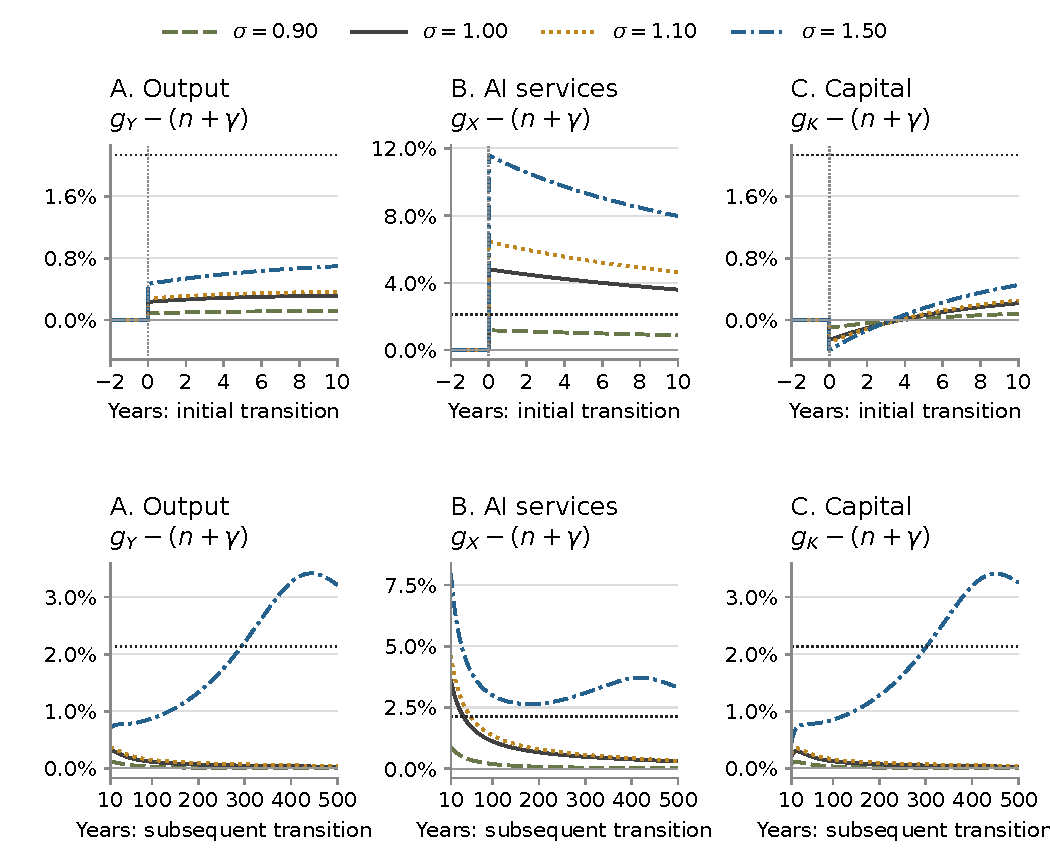
\includegraphics[width=\textwidth]{figures_rewrite/equilibrium_rsi_chi_1_5_accumulation_growth_windows.pdf}
 \caption{Lower research productivity ($\chi=1.5$): growth of output,
 AI production services, and capital per unit of effective labor.
 Rates are instantaneous annual rates. The upper row shows two pre-event
 years and years 0--10; the lower row shows years 10--500. Panels A and C
 share a scale within each row. The vertical line marks RSI activation.}
 \label{fig:rewrite-rsi-research-accumulation}
\end{figure}

\begin{figure}[H]
 \centering
 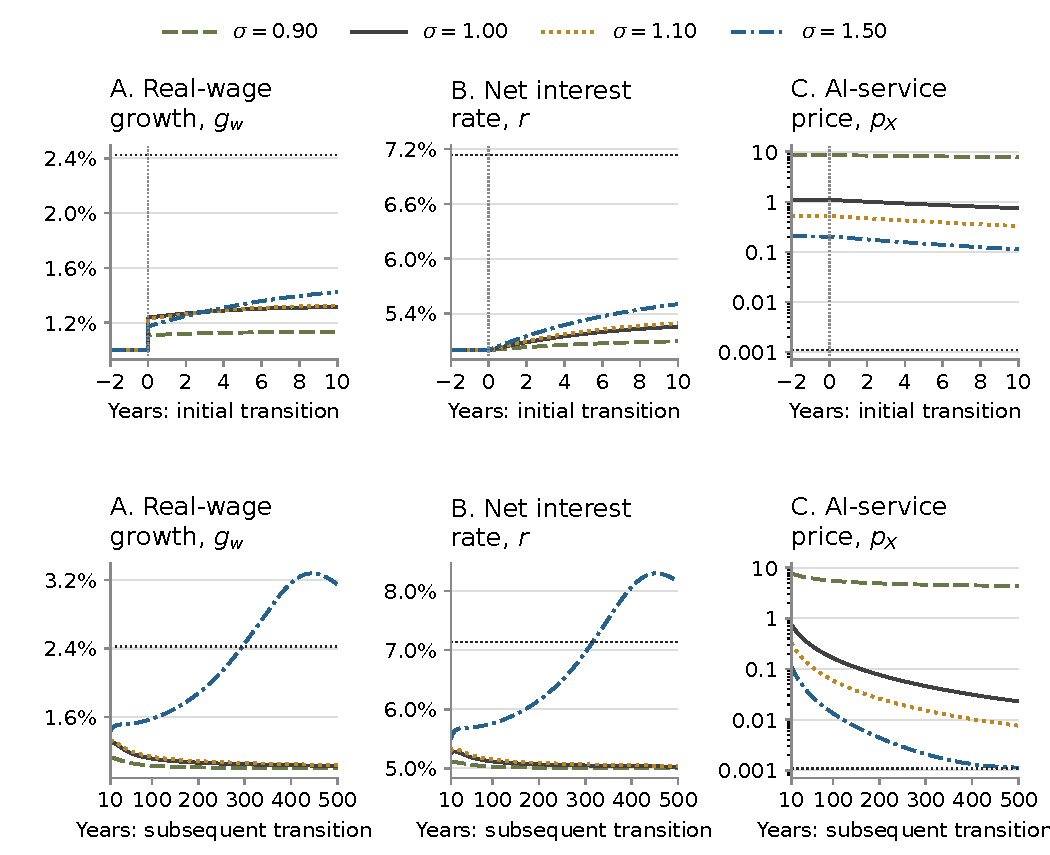
\includegraphics[width=\textwidth]{figures_rewrite/equilibrium_rsi_chi_1_5_growth_returns_windows.pdf}
 \caption{Lower research productivity ($\chi=1.5$): real-wage growth,
 the net interest rate, and the AI-service price. Rates are annual;
 the price is in final-good units on a logarithmic scale.
 The vertical line marks RSI activation.}
 \label{fig:rewrite-rsi-research-prices}
\end{figure}

\begin{figure}[H]
 \centering
 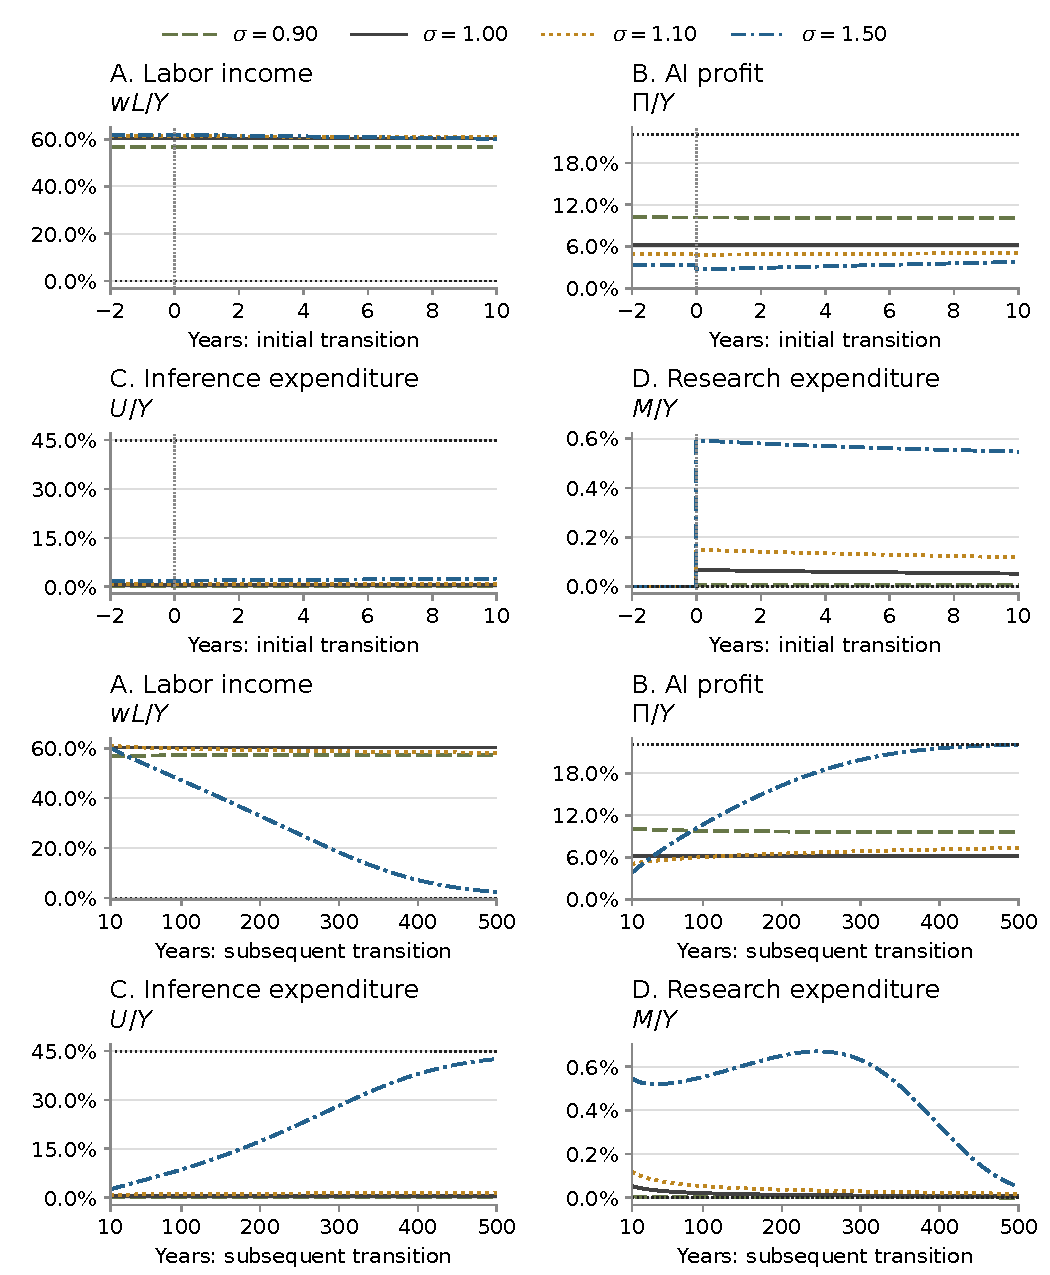
\includegraphics[width=\textwidth]{figures_rewrite/equilibrium_rsi_chi_1_5_ai_distribution_windows.pdf}
 \caption{Lower research productivity ($\chi=1.5$): labor income,
 AI net profit, inference expenditure, and research expenditure relative
 to output. The first two rows show the pre-event BGP and years 0--10;
 the last two show years 10--500. The omitted gross capital share
 remains $\alpha=0.33$.}
 \label{fig:rewrite-rsi-research-distribution}
\end{figure}
